\documentclass{standalone}
\usepackage{tikz}
\begin{document}
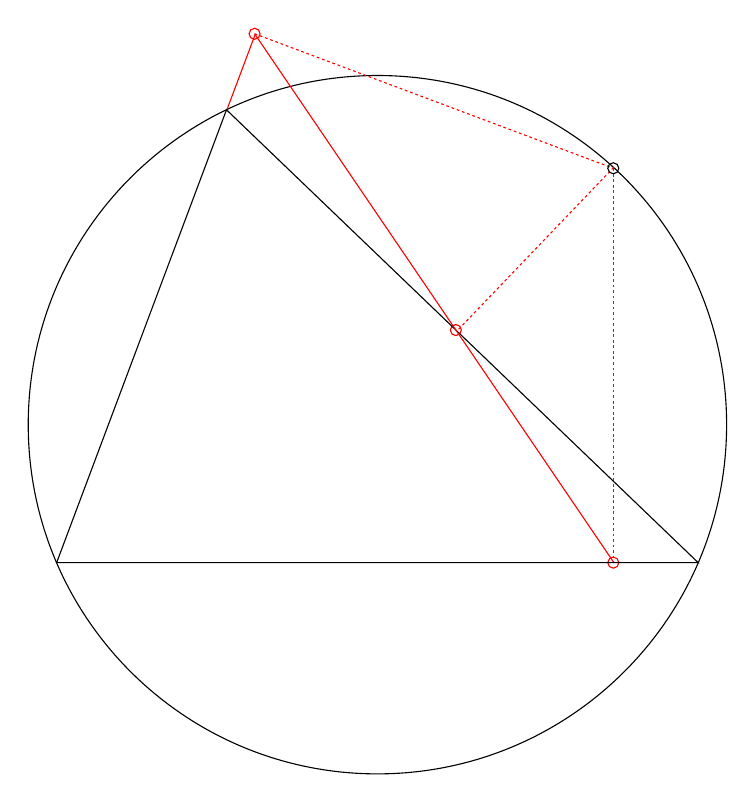
\begin{tikzpicture}[x=1pt,y=1pt]
\draw (136.36,-161.51) circle (126.18);
\draw[red, dash pattern=on 1pt] (221.75,-68.52) -- (165.04,-127.72);
\draw[red, dash pattern=on 1pt] (91.98,-20.25) -- (221.59,-68.86);
\draw[red, dash pattern=on 1pt] (221.59,-68.86) -- (221.59,-211.02);
\draw (221.59,-68.86) circle (2.00);
\draw[red] (164.71,-127.31) circle (2.00);
\draw[red] (91.98,-20.25) circle (2.00);
\draw[red] (221.59,-211.36) circle (2.00);
\draw[red] (82.05,-47.50) -- (92.10,-20.71);
\draw (252.27,-211.36) -- (20.45,-211.36) -- (81.82,-47.73) -- cycle;
\draw[red] (91.98,-20.25) -- (221.59,-211.02);
\end{tikzpicture}
\end{document}
